 \begin{figure}[!h]
\centering
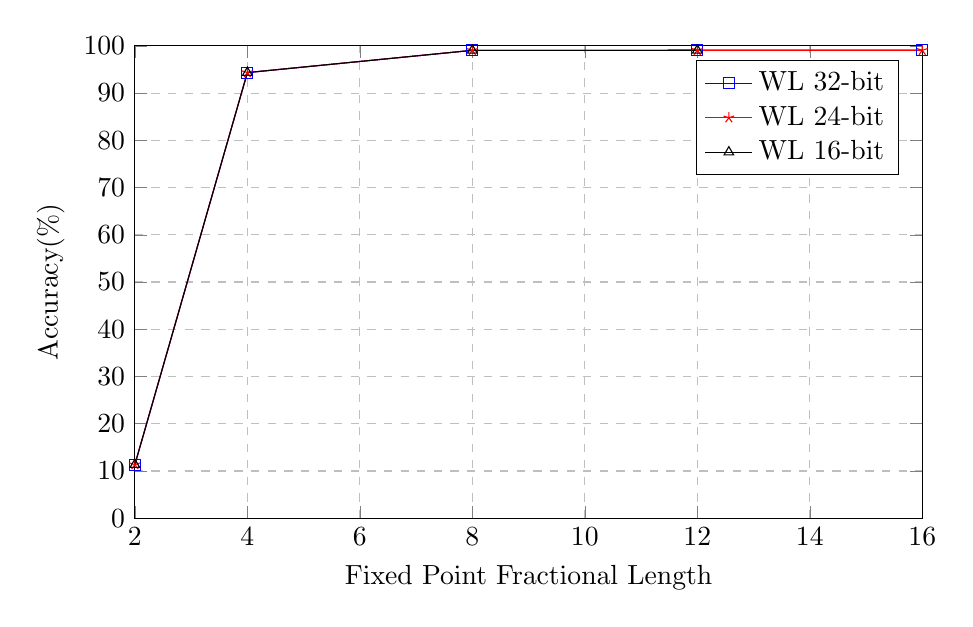
\begin{tikzpicture}
\begin{axis}[
scale only axis,
height=6cm,
width=10cm,
    xlabel={Fixed Point Fractional Length},
    ylabel={Accuracy(\%)},
    xmin=2, xmax=16,
    ymin=0, ymax=100,
    xtick={2,4,6,8,10,12,14,16},
    ytick={0,10,20,30,40,50,60,70,80,90,100},
    legend pos=north east,
    ymajorgrids=true,
    xmajorgrids=true,
    grid style=dashed,
]
\addplot[
    color=blue,
    mark=square,
    ]
    coordinates {
    (2,11.35)(4,94.33)(8,99.04)(12,99.05)(16,99.05)
    };
    \addlegendentry{WL 32-bit}
 \addplot[
    color=red,
    mark=star,
    ]
    coordinates {
    (2,11.35)(4,94.33)(8,99.04)(12,99.05)(16,99.05)
    };
   \addlegendentry{WL 24-bit}
  \addplot[
    color=black,
    mark=triangle,
    ]
    coordinates {
    (2,11.35)(4,94.33)(8,99.04)(12,99.05)
    };
   \addlegendentry{WL 16-bit}
\end{axis}
\end{tikzpicture}
\caption{Effect of varying the Fractional Length on Accuracy}
\label{fig:graph}
\end{figure}